\documentclass{article}
\usepackage{ctex}
\usepackage{geometry}
\usepackage{graphicx}
\usepackage{subcaption}
\usepackage{amsmath}

\title{ResNet-18与CIFAR-100}
\author{王逸群 19307110397}
\date{2022.4.17}

\geometry{a4paper,scale=0.75}

\begin{document}

\maketitle

GitHub repo 链接:https://github.com/quniLcs/cv-mid

网盘链接:

\section{数据集}

本项目使用CIFAR-100数据集,
其中包含60000张$32\times32$的彩色图片,
其中训练集50000张,测试集10000张,
被平均分为100类。

\section{网络结构}

本项目使用ResNet-18网络结构,
其中激活函数为ReLU,
最大的特征为残差连接。
后者包括两种单元结构如图\ref{fig:GraphI}和图\ref{fig:GraphII}所示。

\begin{figure}[p]
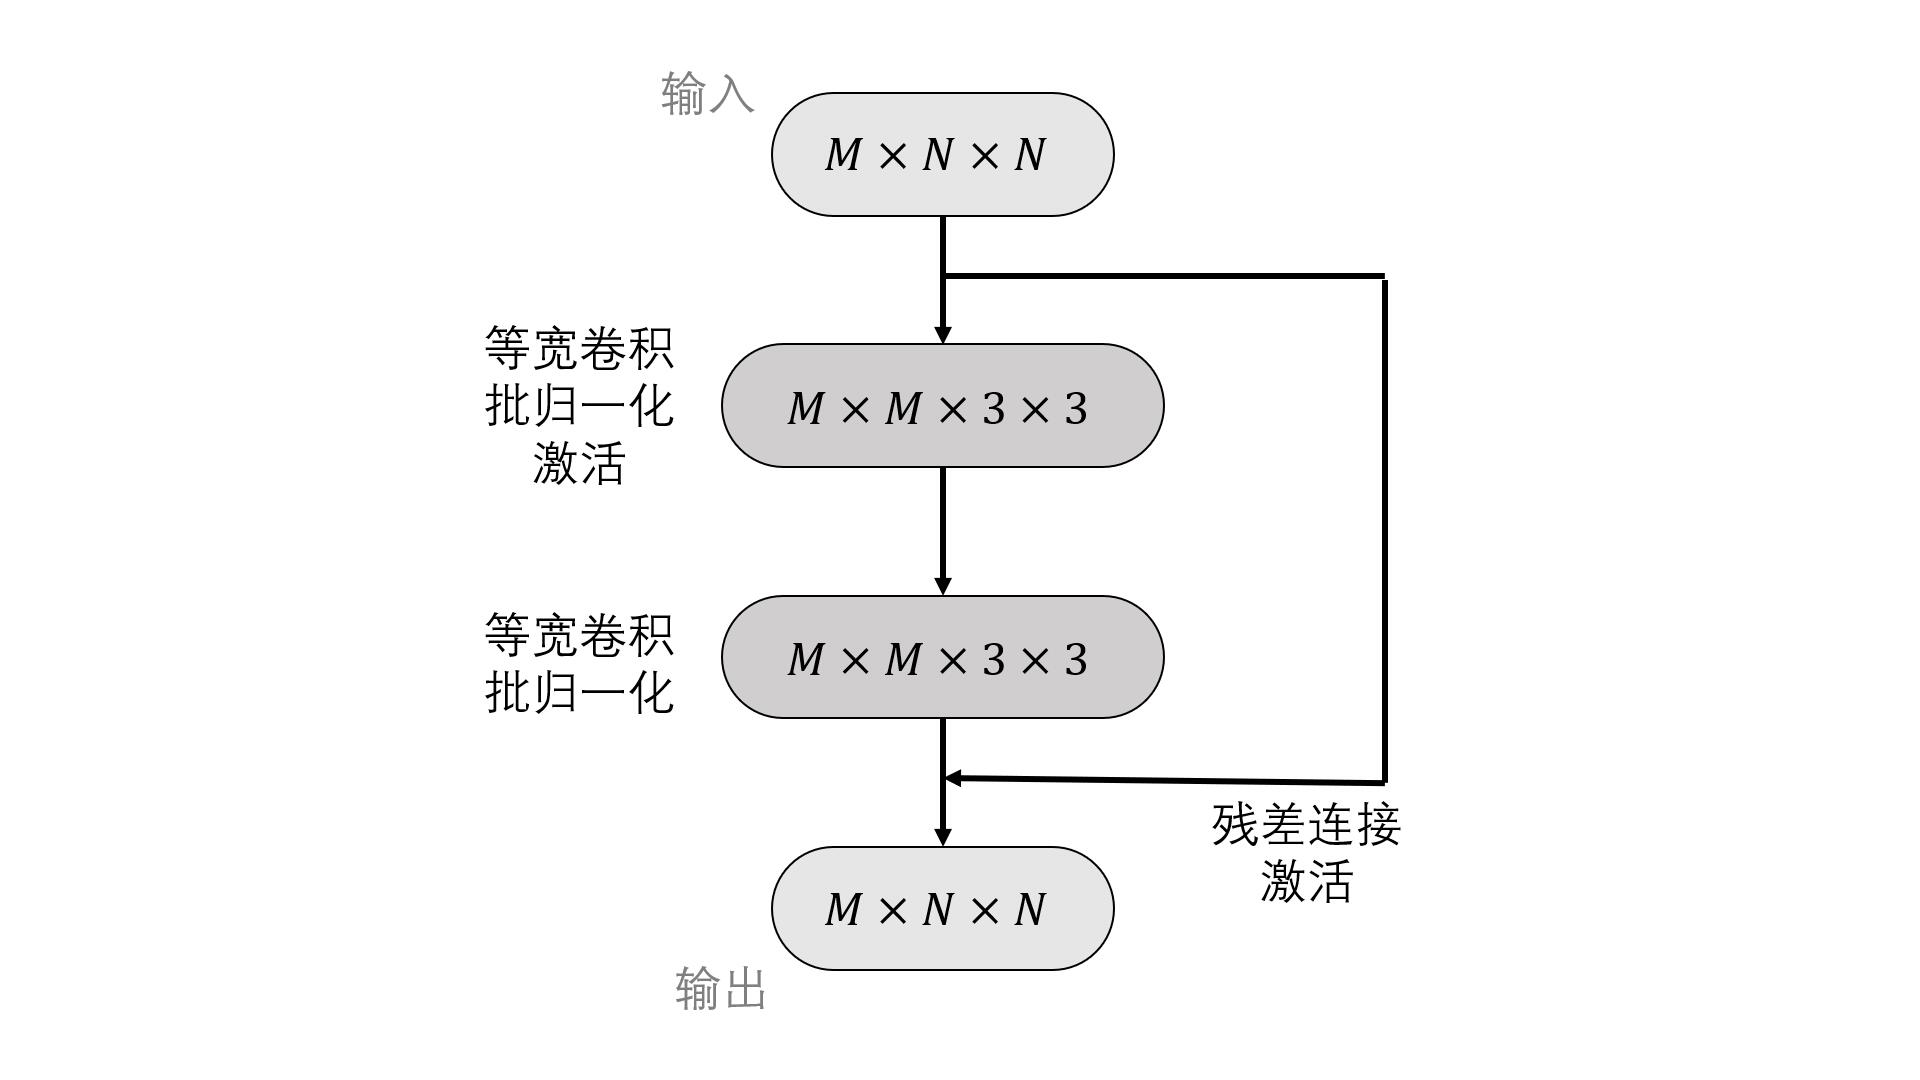
\includegraphics[width=\linewidth]{graph/I.jpg}
\caption{残差连接第一种单元结构}
\label{fig:GraphI}
\end{figure}

\begin{figure}[p]
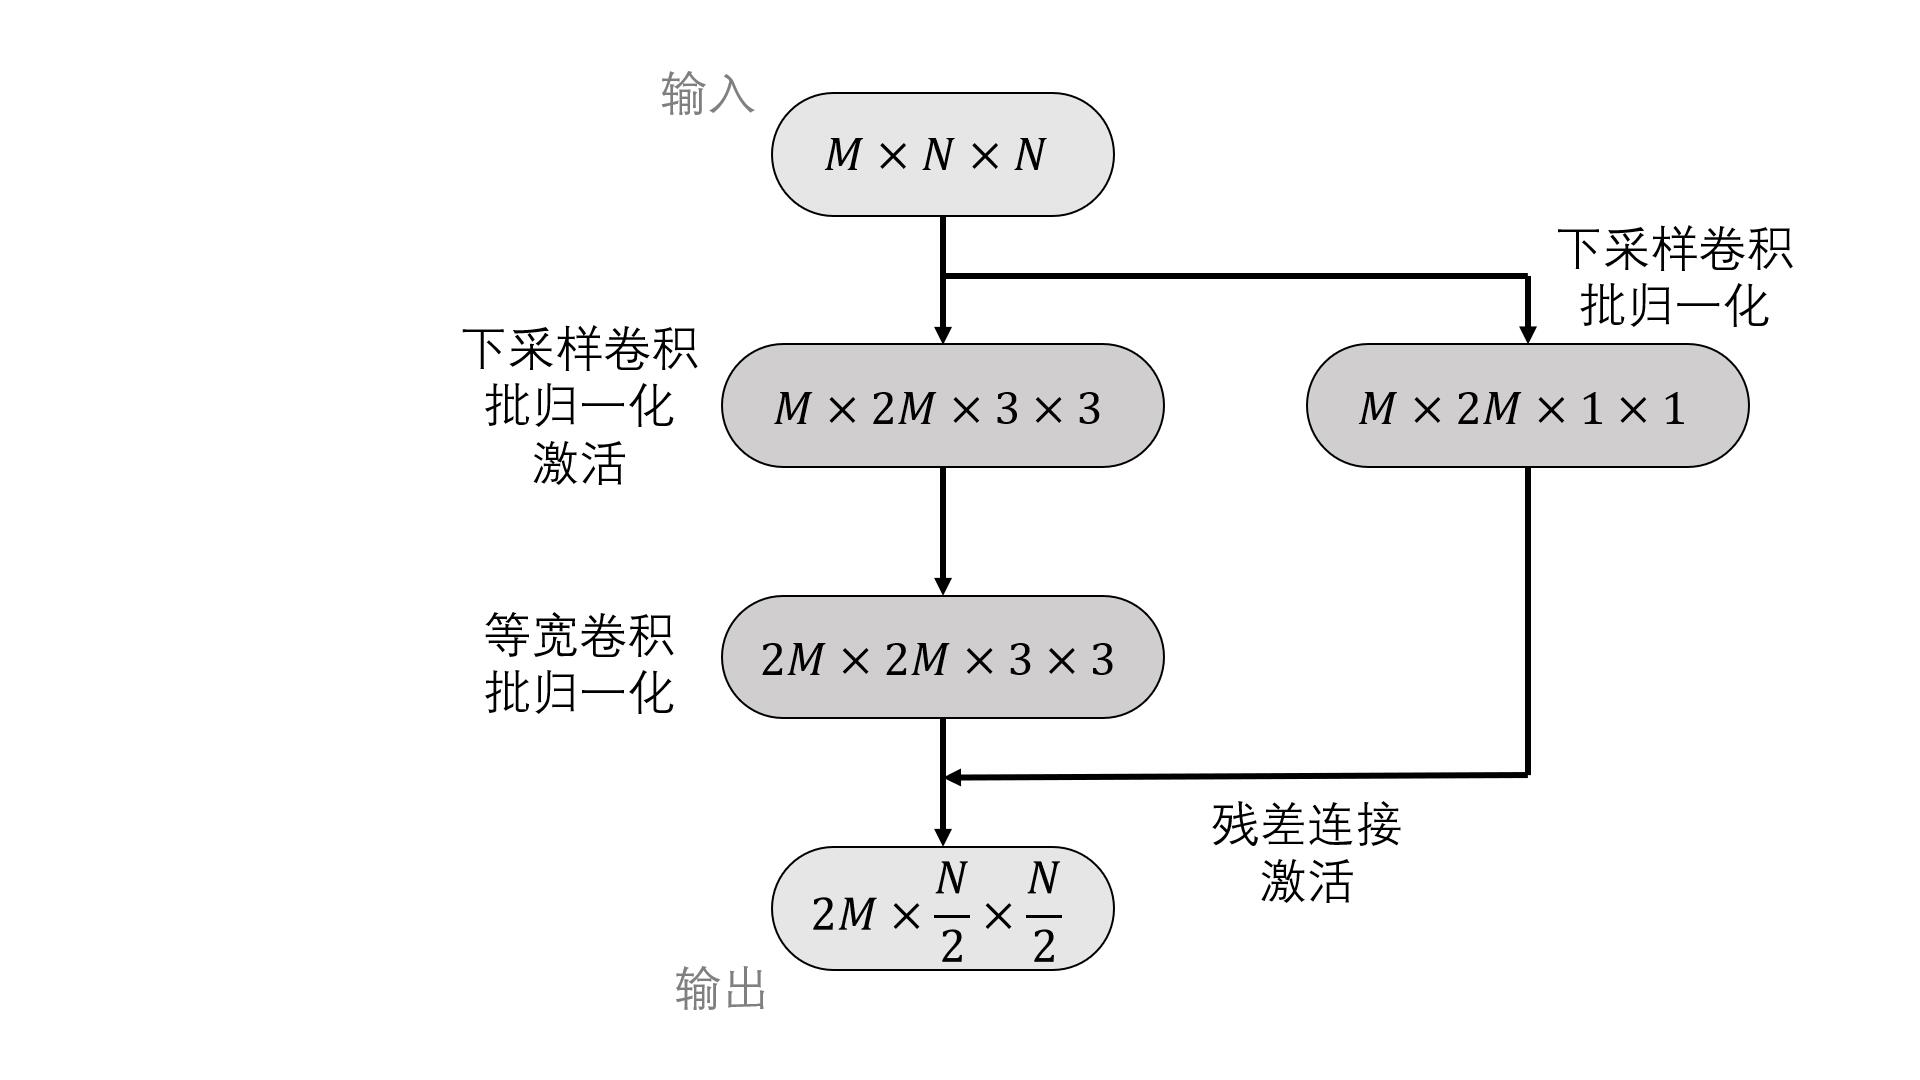
\includegraphics[width=\linewidth]{graph/II.jpg}
\caption{残差连接第二种单元结构}
\label{fig:GraphII}
\end{figure}

对于输入的图像,
先进行步长为1的$3\times64\times3\times3$卷积操作,
并进行批归一化和激活,
维度变为$64\times32\times32$;
接着通过两次第一种单元结构,维度不变;
再通过第二种单元结构,维度变为$128\times16\times16$;
再通过第一种单元结构,维度不变;
再通过第二种单元结构,维度变为$256\times8\times8$;
再通过第一种单元结构,维度不变;
再通过第二种单元结构,维度变为$512\times4\times4$;
再通过第一种单元结构,维度不变;
最后通过全连接得到输出。

\section{超参数设置}

参数初始化:MSRA;

学习率:由0.1开始每10个回合阶梯下降一个数量级;

优化器:带有0.9动量的随机梯度下降算法;

正则化参数:0.0005;

回合数:40;

批量大小:128;

每回合循环数:391;

总循环数:$ 40 \times 391 = 15640$;

损失函数:交叉熵损失函数;

评价指标:精确度。

\section{数据增强}

\subsection{Cutout}

该数据增强方法对于输入的图像,
随机选取一点作为中心点,
将其周围的正方形区域置为0。
具体效果如图\ref{fig:DA}所示。

\subsection{Mixup}

该数据增强方法对一对输入的图像及标签进行凸组合,
凸组合系数服从Beta分布。
具体操作为,
对样本$x_i$、$y_i$、$x_j$、$y_j$,
凸组合系数$\lambda \sim Beta(\alpha, \alpha)$,
产生新的样本和标签:
\begin{align*}
x &= \lambda x_i + (1 - \lambda) x_j \\
y &= \lambda y_i + (1 - \lambda) y_j
\end{align*}

具体效果如图\ref{fig:DA}所示。

\subsection{Cutmix}

该数据增强方法结合了以上两种方法。
具体操作为,
对样本$x_i$、$y_i$、$x_j$、$y_j$,
凸组合系数$\lambda \sim Beta(\alpha, \alpha)$,
先从$ H \times W$的样本$x_i$中随机选取一点作为中心点,
将其周围$ H \sqrt{1 - \lambda} \times W \sqrt{1 - \lambda}$
的正方形区域置为样本$x_j$的值,
即正方形区域面积占比为$ 1 - \lambda $。
由于实际正方形区域可能超出样本区域,
最后将$ \lambda $修正为保留原样本值的区域面积占比,
并产生新的标签:
\begin{align*}
y &= \lambda y_i + (1 - \lambda) y_j
\end{align*}

具体效果如图\ref{fig:DAeffect}所示。

\begin{figure}[h]
\begin{subfigure}{0.19\textwidth}
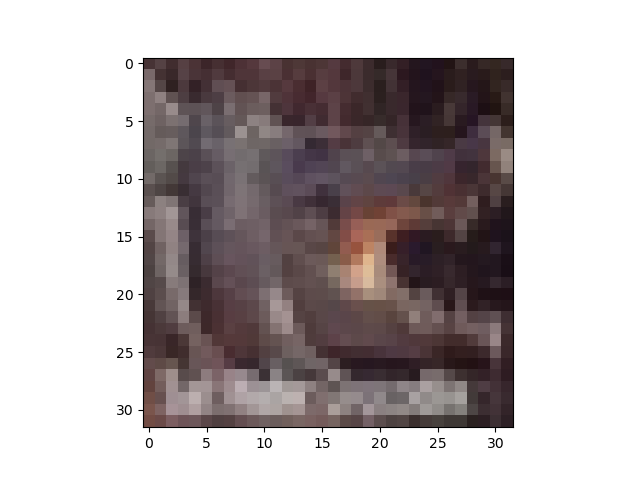
\includegraphics[width=\linewidth]{figure/baseline0.png}
\end{subfigure}
\begin{subfigure}{0.19\textwidth}
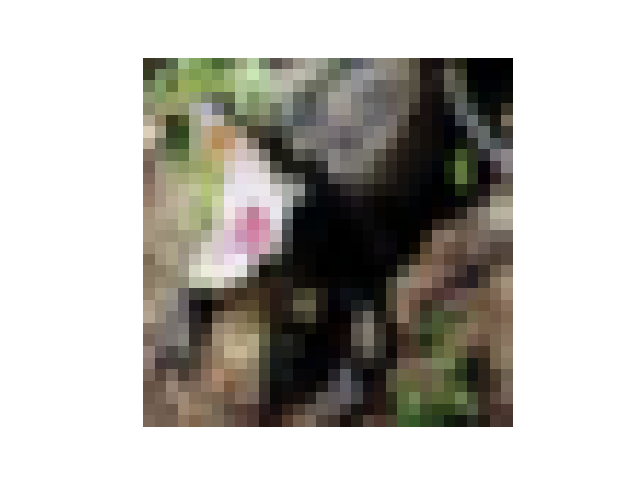
\includegraphics[width=\linewidth]{figure/baseline3.png}
\end{subfigure}
\begin{subfigure}{0.19\textwidth}
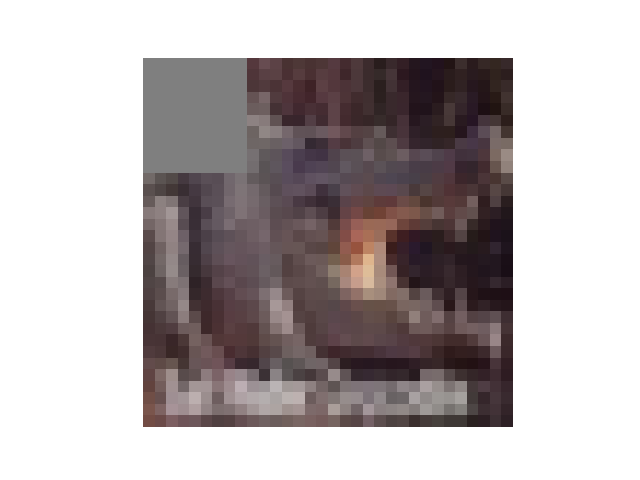
\includegraphics[width=\linewidth]{figure/cutout0.png}
\end{subfigure}
\begin{subfigure}{0.19\textwidth}
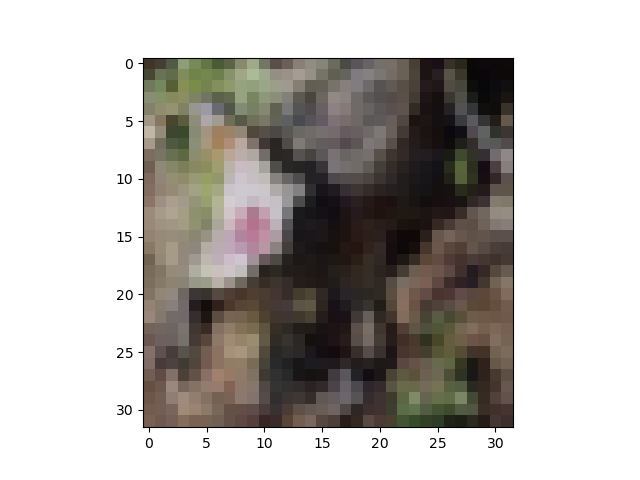
\includegraphics[width=\linewidth]{figure/mixup0.png}
\end{subfigure}
\begin{subfigure}{0.19\textwidth}
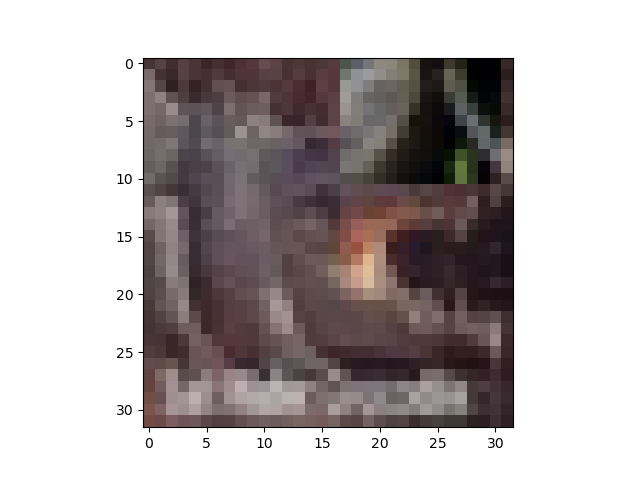
\includegraphics[width=\linewidth]{figure/cutmix0.png}
\end{subfigure}
\begin{subfigure}{0.19\textwidth}
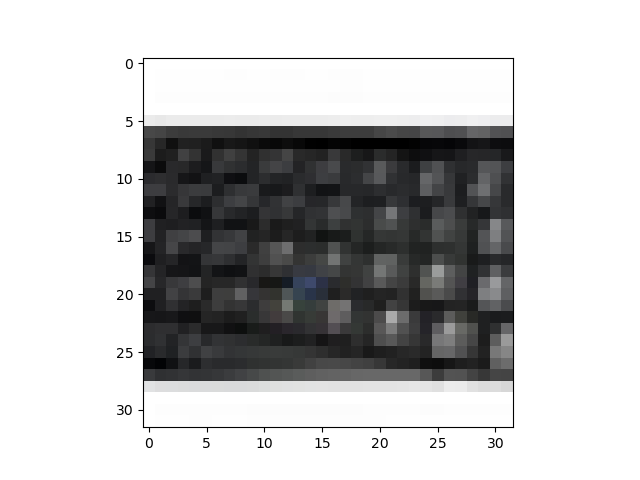
\includegraphics[width=\linewidth]{figure/baseline1.png}
\end{subfigure}
\begin{subfigure}{0.19\textwidth}
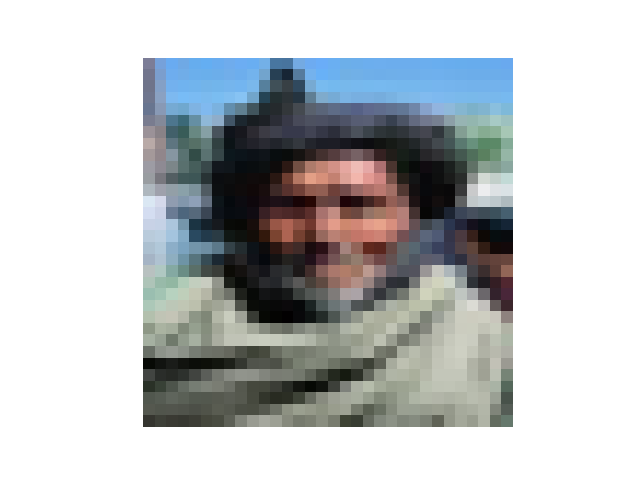
\includegraphics[width=\linewidth]{figure/baseline4.png}
\end{subfigure}
\begin{subfigure}{0.19\textwidth}
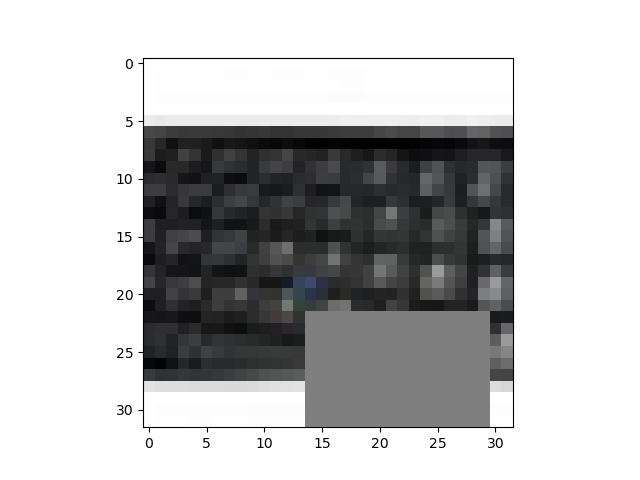
\includegraphics[width=\linewidth]{figure/cutout1.png}
\end{subfigure}
\begin{subfigure}{0.19\textwidth}
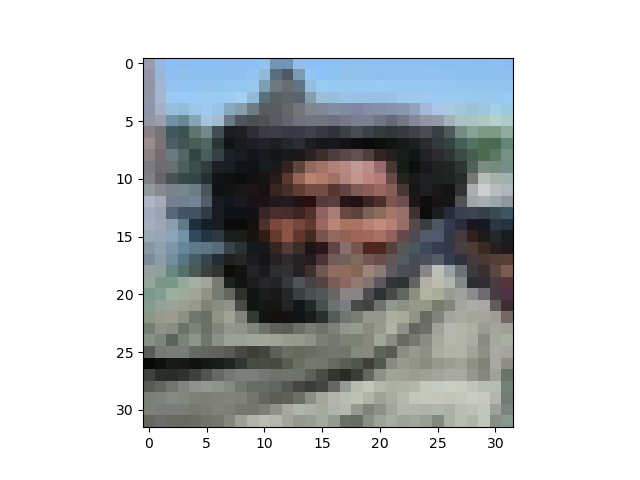
\includegraphics[width=\linewidth]{figure/mixup1.png}
\end{subfigure}
\begin{subfigure}{0.19\textwidth}
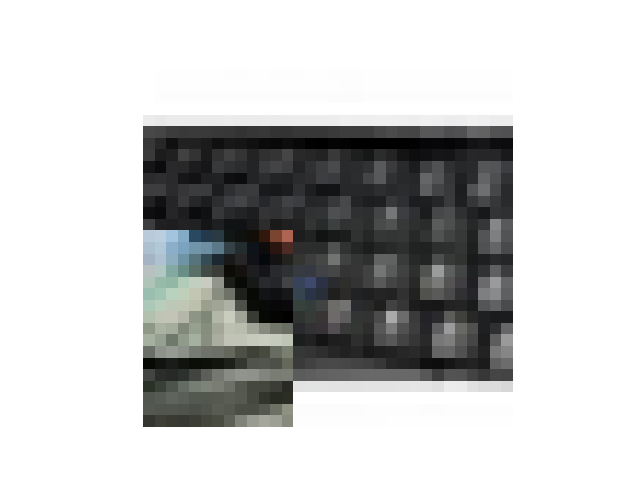
\includegraphics[width=\linewidth]{figure/cutmix1.png}
\end{subfigure}
\begin{subfigure}{0.19\textwidth}
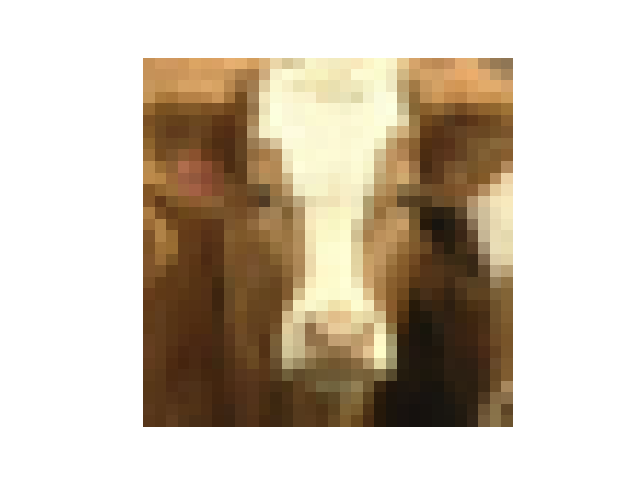
\includegraphics[width=\linewidth]{figure/baseline2.png}
\caption{sample 1}
\end{subfigure}
\begin{subfigure}{0.19\textwidth}
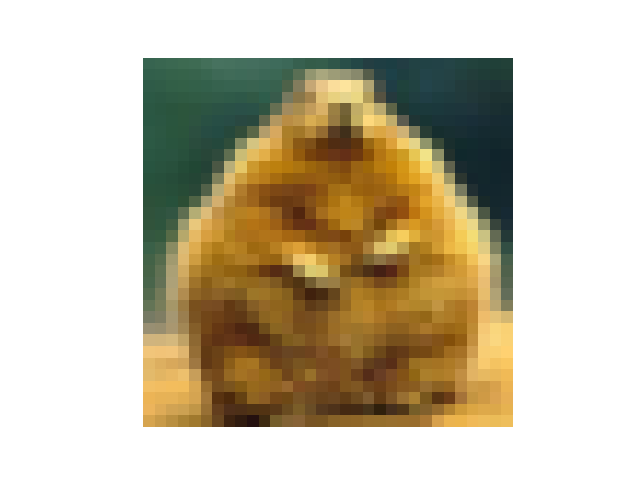
\includegraphics[width=\linewidth]{figure/baseline5.png}
\caption{sample 2}
\end{subfigure}
\begin{subfigure}{0.19\textwidth}
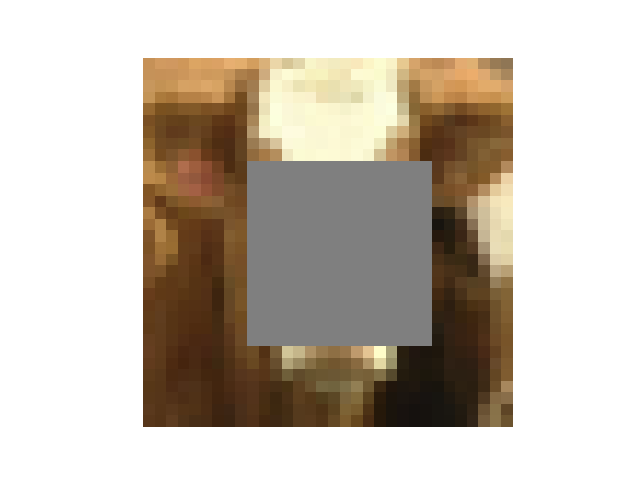
\includegraphics[width=\linewidth]{figure/cutout2.png}
\caption{Cutout}
\end{subfigure}
\begin{subfigure}{0.19\textwidth}
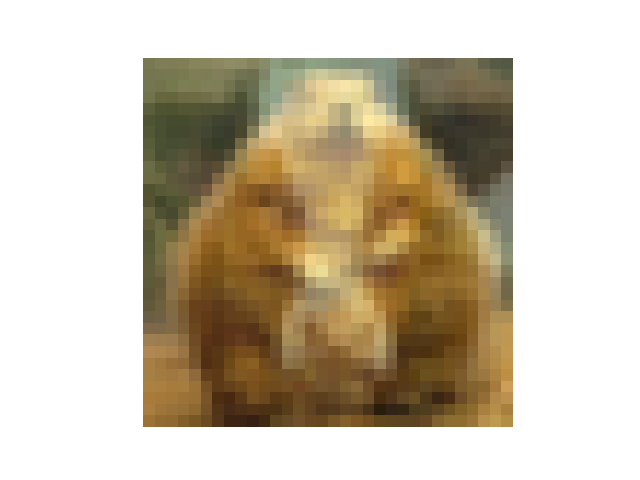
\includegraphics[width=\linewidth]{figure/mixup2.png}
\caption{Mixup}
\end{subfigure}
\begin{subfigure}{0.19\textwidth}
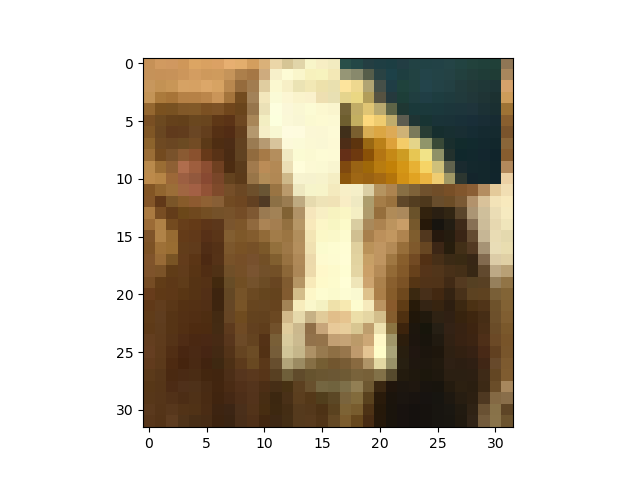
\includegraphics[width=\linewidth]{figure/cutmix2.png}
\caption{CutMix}
\end{subfigure}
\caption{数据增强效果}
\label{fig:DAeffect}
\end{figure}

\section{实验结果}

实验结果如图\ref{fig:DAresult}和表\ref{table:DAresult}所示。

\begin{figure}[h]
\begin{subfigure}{0.5\textwidth}
\includegraphics[width=\linewidth]
{plot/baseline loss legend.png}
\end{subfigure}
\begin{subfigure}{0.5\textwidth}
\includegraphics[width=\linewidth]
{plot/baseline top1 legend.png}
\end{subfigure}
\begin{subfigure}{0.5\textwidth}
\includegraphics[width=\linewidth]
{plot/cutout loss legend.png}
\end{subfigure}
\begin{subfigure}{0.5\textwidth}
\includegraphics[width=\linewidth]
{plot/cutout top1 legend.png}
\end{subfigure}
\begin{subfigure}{0.5\textwidth}
\includegraphics[width=\linewidth]
{plot/mixup loss legend.png}
\end{subfigure}
\begin{subfigure}{0.5\textwidth}
\includegraphics[width=\linewidth]
{plot/mixup top1 legend.png}
\end{subfigure}
\begin{subfigure}{0.5\textwidth}
\includegraphics[width=\linewidth]
{plot/cutmix loss legend.png}
\end{subfigure}
\begin{subfigure}{0.5\textwidth}
\includegraphics[width=\linewidth]
{plot/cutmix top1 legend.png}
\end{subfigure}
\caption{实验结果}
\label{fig:DAresult}
\end{figure}

\begin{table}[h]
\centering
\begin{tabular}{|l|c|c|c|c|} 
\hline
模型 
& 训练集top1精确度 & 训练集top5精确度 
& 测试集top1精确度 & 测试集top5精确度\\
\hline
baseline & 0.99982 & 1.00000 & 0.61110 & 0.84930 \\
Cutout   & 0.99982 & 1.00000 & 0.65360 & 0.87540 \\
Mixup    & 0.99980 & 1.00000 & 0.60050 & 0.81830 \\
CutMix   & 0.99980 & 1.00000 & 0.63310 & 0.85980 \\
\hline
\end{tabular}
\caption{实验结果}
\label{table:DAresult}
\end{table}

可以看到,
模型训练的难点在于,
训练集的精确度快速达到近乎100\%,
测试集的精确度便不再有上升的空间。
数据增强的意义在于,
加大训练集收敛的难度,
使得测试集有更大的提升机会。

例如,在第15个回合,
baseline模型的训练集精确率达到了0.75324,
但测试集精确率仅有0.46340;
相比之下,
cutout模型的训练集精确率仅有0.69558,
但测试集精确率有0.51210。

最后,mixup对模型没有明显提升,cutmix和cutout都优化了模型结果。

\end{document}